\documentclass[11pt,a4paper]{article}

\usepackage[T1]{fontenc}
\usepackage[utf8]{inputenc}
\usepackage[brazil]{babel}
\usepackage{lmodern}
\usepackage{microtype}
\usepackage{geometry}
\geometry{margin=25mm}
\usepackage{amsmath,amssymb,bm,mathtools}
\usepackage{siunitx}
\sisetup{per-mode=symbol}
\usepackage{booktabs,tabularx,array}
\usepackage{xcolor}
\usepackage{graphicx}
\usepackage{tikz}
\usetikzlibrary{arrows.meta,angles,quotes,calc}
\usepackage{listings}
\usepackage{fancyhdr}
\usepackage{hyperref}
\usepackage[nameinlink,noabbrev]{cleveref}

\definecolor{navy}{HTML}{17365D}
\definecolor{blue}{HTML}{2E75B6}
\definecolor{lightblue}{HTML}{D9EAF7}
\definecolor{codegreen}{HTML}{287A3D}
\definecolor{codegray}{HTML}{5B6573}
\hypersetup{colorlinks=true,linkcolor=navy,urlcolor=blue,citecolor=navy}

\pagestyle{fancy}
\fancyhf{}
\lhead{Dinâmica não linear}
\rhead{Pêndulo em disco rotativo}
\cfoot{\thepage}
\setlength{\headheight}{14pt}

\lstdefinestyle{matlab}{
  language=Matlab,
  basicstyle=\ttfamily\small,
  keywordstyle=\color{blue}\bfseries,
  commentstyle=\color{codegreen},
  stringstyle=\color{purple},
  numbers=left,
  numberstyle=\tiny\color{codegray},
  frame=single,
  rulecolor=\color{lightblue},
  breaklines=true,
  showstringspaces=false,
  columns=fullflexible,
  keepspaces=true
}

\newcommand{\bvec}[1]{\bm{#1}}
\newcommand{\R}[2]{{}^{#1}\!\bvec R_{#2}}
\newcommand{\vct}[2]{{}^{#1}\!\bvec{#2}}

\title{\textbf{Dinâmica de um Pêndulo Montado em Disco Rotativo}\\
\large Modelagem, integração numérica e validação computacional}
\author{Everton Machado do Amparo}
\date{\today}

\begin{document}
\maketitle

\begin{abstract}
Este trabalho estuda um pêndulo montado na extremidade de um braço e sobre um
disco rotativo. O exercício usado como referência considera velocidades
angulares constantes; aqui, essa hipótese é mantida como caso de verificação e
depois substituída por movimentos prescritos $\alpha(t)$ e $\beta(t)$ com
velocidades e acelerações variáveis. A formulação resultante é implementada em
MATLAB, Simulink e Simscape Multibody. O código inclui um integrador de
Runge--Kutta de quarta ordem, comparação com \texttt{ode45}, testes de
consistência cinemática e confronto entre o modelo por equações e o modelo
multicorpos. A geometria foi escrita de modo a permitir a futura substituição
dos sólidos paramétricos por componentes CAD.
\end{abstract}

\tableofcontents

\section{Escopo da modelagem}

O enunciado usado como ponto de partida impõe velocidades angulares constantes
ao braço e ao disco. Sob essa hipótese,
$\ddot\alpha=\ddot\beta=0$. O modelo desenvolvido neste trabalho é mais geral:
$\alpha(t)$ e $\beta(t)$ são funções prescritas, com derivadas conhecidas até a
segunda ordem. Define-se
\begin{equation}
\Omega(t)=\dot\alpha(t)+\dot\beta(t), \qquad
\dot\Omega(t)=\ddot\alpha(t)+\ddot\beta(t), \qquad
\rho=r+l\sin\psi.
\label{eq:definitions}
\end{equation}

A equação de movimento obtida para a coordenada livre $\psi$ é
\begin{equation}
\boxed{
l\ddot\psi+g\sin\psi
+b\left(\dot\alpha^{\,2}\sin\beta+\ddot\alpha\cos\beta\right)\cos\psi
-\Omega^2\left(r+l\sin\psi\right)\cos\psi=0.}
\label{eq:eom}
\end{equation}
O termo com $\ddot\alpha$ representa a aceleração tangencial do ponto $B$. A
aceleração $\ddot\beta$ não aparece diretamente em \cref{eq:eom}: para a
geometria adotada, a aceleração de Euler associada a $\dot\Omega$ atua em
$X_2$, perpendicular ao plano de oscilação. Ela permanece, porém, na aceleração
absoluta de $E$ e nas reações da junta.

Quando $\dot\alpha$ e $\dot\beta$ são constantes, a expressão anterior se reduz
ao resultado do exercício de referência:
\begin{equation}
 l\ddot\psi+g\sin\psi
 +b\dot\alpha^{\,2}\sin\beta\cos\psi
 -(\dot\alpha+\dot\beta)^2\left(r+l\sin\psi\right)\cos\psi=0.
\label{eq:eom-constant-rate}
\end{equation}
Essa coincidência verifica o caso particular, sem estender a conclusão a todas
as etapas da resolução manuscrita.

As seguintes convenções geométricas são usadas em todo o projeto:
\begin{enumerate}
  \item $r$ é a distância radial, no plano do disco, entre o eixo em $C$ e o
  pivô em $D$;
  \item $h$ é a distância vertical de $C$ a $D$. Assim, a coordenada vertical
  de $B$ a $D$ é $c+h$, e a de $O$ a $D$ é $a+c+h$;
  \item $a$, $c$ e $h$ são deslocamentos verticais constantes: afetam a posição
  absoluta, mas não a equação dinâmica ideal;
  \item $\Omega$ é a velocidade angular absoluta do disco, pois os giros de
  $\alpha$ e $\beta$ ocorrem em torno de eixos verticais paralelos.
\end{enumerate}
\section{Descrição física e hipóteses}

O referencial inercial $I$ tem origem em $O$. As bases móveis $B1$, $B2$ e $B3$
têm origens em $B$, $C$ e $D$, respectivamente. A base $B1$ é solidária ao
braço, $B2$ ao disco e $B3$ à haste. A massa $m$ é concentrada na partícula $E$.

\begin{figure}[ht]
\centering
\begin{tikzpicture}[>=Latex,scale=0.95,every node/.style={font=\small}]
  % top view
  \begin{scope}[xshift=-4.8cm]
    \node[font=\bfseries] at (1.7,3.0) {Vista superior};
    \coordinate (A) at (0,0);
    \coordinate (B) at (3,0);
    \coordinate (D) at (3,1.8);
    \fill (A) circle (2pt) node[below left] {$A$};
    \fill (B) circle (2pt) node[below right] {$B$ ($C$ em projeção)};
    \fill (D) circle (2pt) node[above right] {$D$};
    \draw[very thick,navy] (A)--node[below] {$b$}(B);
    \draw[very thick,blue] (B)--node[right] {$r$}(D);
    \draw[->] (A)--++(1.2,0) node[below] {$\bvec i_1$};
    \draw[->] (B)--++(0,1.2) node[left] {$\bvec j_2$};
    \draw[dashed] (A)--++(0,2.2);
    \draw[->] ($(A)+(0,0.65)$) arc[start angle=90,end angle=25,radius=0.65];
    \node at (0.65,0.75) {$\alpha$};
    \draw[->] ($(B)+(0.65,0)$) arc[start angle=0,end angle=70,radius=0.65];
    \node at (3.75,0.65) {$\beta$};
  \end{scope}
  % vertical section
  \begin{scope}[xshift=2.1cm]
    \node[font=\bfseries] at (2.0,3.0) {Seção no plano $Y_2Z_2$};
    \coordinate (C2) at (0,0);
    \coordinate (P2) at (2.1,0);
    \coordinate (D2) at (2.1,1.1);
    \coordinate (E2) at (3.2,-1.15);
    \fill (C2) circle (2pt) node[below left] {$C$};
    \fill (D2) circle (2pt) node[above] {$D$};
    \fill (E2) circle (3pt) node[right] {$E,m$};
    \draw[very thick,blue] (C2)--node[below] {$r$}(P2);
    \draw[very thick,blue] (P2)--node[right] {$h$}(D2);
    \draw[very thick,navy] (D2)--node[right] {$l$}(E2);
    \draw[dashed] (D2)--++(0,-2.6);
    \draw[->] (C2)--++(3.8,0) node[right] {$Y_2$};
    \draw[->] (C2)--++(0,2.0) node[above] {$Z_2$};
    \draw[->] ($(D2)+(0,-0.75)$) arc[start angle=-90,end angle=-64,radius=0.75];
    \node at (2.35,0.20) {$\psi$};
    \draw[<->,gray] (D2)--node[above] {$l\sin\psi$}(3.2,1.1);
  \end{scope}
\end{tikzpicture}
\caption{Esquema autoral simplificado. Na vista superior, $B$ e $C$ têm a
mesma projeção horizontal, mas são separados pelo deslocamento vertical $c$.
O raio instantâneo da massa em relação ao eixo do disco é
$\rho=r+l\sin\psi$; sua altura absoluta inclui $a+c+h$.}
\label{fig:geometry}
\end{figure}

As hipóteses do modelo-base são:
\begin{itemize}
  \item haste rígida e sem massa; partícula $E$ pontual;
  \item vínculos ideais e ausência de folgas;
  \item gravidade uniforme, $\bvec g=-g\bvec k$;
  \item $\alpha(t)$ e $\beta(t)$ impostas por atuadores ideais, com derivadas
  conhecidas até a segunda ordem;
  \item ausência de amortecimento e torque externo na formulação ideal.
\end{itemize}

Os vetores geométricos são
\begin{align}
\vct{B1}{r}_{AB}&=\begin{bmatrix}b&0&0\end{bmatrix}^{\!T}, &
\vct{B1}{r}_{BC}&=\begin{bmatrix}0&0&c\end{bmatrix}^{\!T},\\
\vct{B2}{r}_{CD}&=\begin{bmatrix}0&r&h\end{bmatrix}^{\!T}, &
\vct{B3}{r}_{DE}&=\begin{bmatrix}0&0&-l\end{bmatrix}^{\!T}.
\end{align}

\section{Transformações de coordenadas}

Adota-se a convenção passiva: $\R{A}{B}$ transforma componentes expressas em
$B$ para componentes expressas em $A$. Assim,
\begin{align}
\R{B1}{I}&=
\begin{bmatrix}
\cos\alpha&\sin\alpha&0\\-\sin\alpha&\cos\alpha&0\\0&0&1
\end{bmatrix},\\
\R{B2}{B1}&=
\begin{bmatrix}
\cos\beta&\sin\beta&0\\-\sin\beta&\cos\beta&0\\0&0&1
\end{bmatrix},\\
\R{B3}{B2}&=
\begin{bmatrix}
1&0&0\\0&\cos\psi&\sin\psi\\0&-\sin\psi&\cos\psi
\end{bmatrix}.
\label{eq:rotations}
\end{align}
Para retornar ao referencial inercial, usa-se a transposta da matriz composta,
pois matrizes de rotação são ortogonais.

\section{Velocidades e acelerações angulares}

Com as definições de \cref{eq:definitions}, as velocidades angulares são
\begin{align}
\vct{B1}{\omega}_1&=\begin{bmatrix}0&0&\dot\alpha\end{bmatrix}^{T},\\
\vct{B2}{\omega}_2&=\begin{bmatrix}0&0&\Omega\end{bmatrix}^{T},\\
\vct{B3}{\omega}_3&=
\begin{bmatrix}\dot\psi&\Omega\sin\psi&\Omega\cos\psi\end{bmatrix}^{T}.
\end{align}
Não se impõe constância às taxas. As acelerações angulares absolutas ficam
\begin{align}
\vct{B1}{\dot\omega}_1&=\begin{bmatrix}0&0&\ddot\alpha\end{bmatrix}^{T},\\
\vct{B2}{\dot\omega}_2&=\begin{bmatrix}0&0&\dot\Omega\end{bmatrix}^{T},\\
\vct{B3}{\dot\omega}_3&=
\begin{bmatrix}
\ddot\psi &
\dot\Omega\sin\psi+\Omega\dot\psi\cos\psi &
\dot\Omega\cos\psi-\Omega\dot\psi\sin\psi
\end{bmatrix}^{T}.
\end{align}
Os termos com $\dot\Omega$ desaparecem apenas no caso particular de velocidades
prescritas constantes.
\section{Aceleração linear da partícula}

A aceleração do ponto $B$, expressa em $B1$, contém parcelas normal e
tangencial:
\begin{equation}
\vct{B1}{a}_B=
\begin{bmatrix}-b\dot\alpha^2&b\ddot\alpha&0\end{bmatrix}^{T}.
\end{equation}
Os deslocamentos $BC=c\bvec k$ e $h\bvec k_2$ são paralelos aos eixos de
rotação. Portanto, $\bvec a_C=\bvec a_B$. Em $B2$,
\begin{equation}
\vct{B2}{a}_C=
\begin{bmatrix}
-b\dot\alpha^2\cos\beta+b\ddot\alpha\sin\beta\\
b\dot\alpha^2\sin\beta+b\ddot\alpha\cos\beta\\0
\end{bmatrix}.
\end{equation}

Usando $\rho=r+l\sin\psi$ e somando as parcelas relativa, de Coriolis,
centrípeta e de Euler, obtém-se
\begin{equation}
\vct{B2}{a}_E=
\begin{bmatrix}
-b\dot\alpha^2\cos\beta+b\ddot\alpha\sin\beta
-\dot\Omega\rho-2l\Omega\dot\psi\cos\psi\\
b\dot\alpha^2\sin\beta+b\ddot\alpha\cos\beta-\Omega^2\rho
+l\ddot\psi\cos\psi-l\dot\psi^2\sin\psi\\
l\ddot\psi\sin\psi+l\dot\psi^2\cos\psi
\end{bmatrix}.
\label{eq:acceleration-b2}
\end{equation}
A primeira componente mostra onde $\ddot\beta$ atua: ela está contida em
$\dot\Omega\rho$. Esse termo é relevante para a reação transversal do pivô,
embora não se projete na direção generalizada de $\psi$.

Definindo
\begin{equation}
A_C=b\left(\dot\alpha^2\sin\beta+\ddot\alpha\cos\beta\right),
\label{eq:arm-acceleration}
\end{equation}
as componentes usadas no diagrama de corpo livre são
\begin{align}
\vct{B3}{a}_{E,y}&=A_C\cos\psi+l\ddot\psi
-\Omega^2\rho\cos\psi,\label{eq:ay3}\\
\vct{B3}{a}_{E,z}&=-A_C\sin\psi+l\dot\psi^2
+\Omega^2\rho\sin\psi.\label{eq:az3}
\end{align}
\section{Diagrama de corpo livre e equação de movimento}

Sobre a partícula atuam a tração $T\bvec k_3$ e o peso. Em $B3$,
\begin{equation}
\vct{B3}{F}=
\begin{bmatrix}0\\-mg\sin\psi\\T-mg\cos\psi\end{bmatrix}.
\end{equation}
Na direção $Y_3$, a segunda lei de Newton combinada com \cref{eq:ay3} produz
\cref{eq:eom}. Na direção $Z_3$, resulta
\begin{equation}
\boxed{T=m\left[g\cos\psi-A_C\sin\psi
+\Omega^2\rho\sin\psi+l\dot\psi^2\right].}
\label{eq:tension}
\end{equation}
Se \cref{eq:tension} fornecer $T<0$, um fio real ficaria frouxo. O modelo atual
usa uma haste rígida ou, de forma equivalente, pressupõe um vínculo sempre
tracionado; perda e retomada de contato exigem outra formulação.
\section{Forma de estado e extensão não ideal}

Com $x_1=\psi$ e $x_2=\dot\psi$, define-se
\begin{equation}
A_C(t)=b\left[\dot\alpha(t)^2\sin\beta(t)
+\ddot\alpha(t)\cos\beta(t)\right].
\end{equation}
A forma de estado ideal é
\begin{align}
\dot x_1&=x_2,\\
\dot x_2&=\frac{1}{l}\left[
\Omega(t)^2(r+l\sin x_1)\cos x_1-g\sin x_1-A_C(t)\cos x_1
\right].
\label{eq:state}
\end{align}
O código admite amortecimento viscoso $d$ no pivô e torque aplicado
$\tau(t,\bvec x)$. Nesse caso,
\begin{equation}
l\ddot\psi+g\sin\psi+A_C\cos\psi
-\Omega^2\rho\cos\psi
+\frac{d}{ml}\dot\psi-\frac{\tau}{ml}=0.
\end{equation}

A linearização em torno de $\psi\approx0$ fornece
\begin{equation}
l\ddot\psi+(g-l\Omega^2)\psi=\Omega^2r-A_C.
\end{equation}
Como $\Omega$ e $A_C$ podem variar, tanto a rigidez efetiva quanto a excitação
são funções do tempo. A aproximação é útil perto da vertical, mas não substitui
o modelo não linear em amplitudes maiores.

\subsection{Lei de movimento usada no caso demonstrativo}

Para manter posição, velocidade e aceleração mutuamente consistentes, cada
ângulo prescrito usa o perfil
\begin{equation}
q(t)=q_0+\bar\omega t+A\left[\sin(\nu t+\phi)-\sin\phi\right],
\end{equation}
com
\begin{equation}
\dot q=\bar\omega+A\nu\cos(\nu t+\phi), \qquad
\ddot q=-A\nu^2\sin(\nu t+\phi).
\end{equation}
Esse perfil serve apenas como entrada reproduzível. Em MATLAB, ele pode ser
substituído por uma função que devolva
$[\alpha,\dot\alpha,\ddot\alpha,\beta,\dot\beta,\ddot\beta]^T$.
No Simulink e no Multibody, os seis sinais aparecem de forma explícita para que
possam ser trocados por trajetórias medidas, tabeladas ou geradas por um
controlador.
\section{Integração numérica}

Para um sistema genérico $\dot{\bvec x}=\bvec f(t,\bvec x)$, o RK4 clássico usa
\begin{align}
\bvec k_1&=\bvec f(t_n,\bvec x_n),\\
\bvec k_2&=\bvec f(t_n+\tfrac{\Delta t}{2},
\bvec x_n+\tfrac{\Delta t}{2}\bvec k_1),\\
\bvec k_3&=\bvec f(t_n+\tfrac{\Delta t}{2},
\bvec x_n+\tfrac{\Delta t}{2}\bvec k_2),\\
\bvec k_4&=\bvec f(t_n+\Delta t,\bvec x_n+\Delta t\bvec k_3),\\
\bvec x_{n+1}&=\bvec x_n+\frac{\Delta t}{6}
(\bvec k_1+2\bvec k_2+2\bvec k_3+\bvec k_4).
\end{align}
O erro global é de ordem $\mathcal O(\Delta t^4)$. O projeto compara esse
integrador de passo fixo com o \texttt{ode45}, um método adaptativo adequado
como referência para este problema não rígido. Se o modelo futuro incluir
contato muito rígido, saturações rápidas ou flexibilidade estrutural, devem ser
avaliados \texttt{ode15s} e métodos próprios para sistemas multicorpos.

\section{Arquitetura MATLAB}

O código separa responsabilidades:
\begin{itemize}
  \item \texttt{+rotpend}: parâmetros, equação de estado, cinemática e simulação;
  \item \texttt{+numerics}: integrador RK4 genérico, sem dependência do modelo;
  \item \texttt{+post}: gráficos e trajetória absoluta;
  \item \texttt{tests}: casos-limite, resíduo e convergência;
  \item \texttt{run\_simulation.m}: configuração reproduzível e exportação.
\end{itemize}

A implementação direta da equação de estado é:
\lstinputlisting[style=matlab,caption={Função do lado direito do sistema não linear.},
label={lst:rhs}]{../matlab/+rotpend/rhs.m}

O integrador educacional é independente do pêndulo:
\lstinputlisting[style=matlab,caption={Runge--Kutta clássico de quarta ordem.},
label={lst:rk4}]{../matlab/+numerics/rk4.m}

\section{Validação e rastreabilidade}

Antes de comparar com CAD ou bancada, recomenda-se a seguinte sequência:
\begin{enumerate}
  \item \textbf{Unidades:} todos os termos de \cref{eq:eom} têm unidade de
  aceleração, \si{m.s^{-2}}.
  \item \textbf{Caso-limite:} com $\dot\alpha=\dot\beta=0$ e
  $\ddot\alpha=\ddot\beta=0$, recupera-se
  $\ddot\psi=-(g/l)\sin\psi$.
  \item \textbf{Resíduo:} substituir a aceleração calculada na equação e exigir
  resíduo próximo da precisão de máquina.
  \item \textbf{Convergência:} reduzir $\Delta t$ à metade; no regime assintótico,
  o erro do RK4 deve cair aproximadamente por um fator 16.
  \item \textbf{Solver cruzado:} comparar RK4 e \texttt{ode45} nos mesmos
  instantes de amostragem.
  \item \textbf{Vínculo:} verificar numericamente
  $\lVert\bvec r_E-\bvec r_D\rVert=l$ e monitorar $T\ge0$.
  \item \textbf{Modelo 3D:} comparar posição, velocidade e aceleração de $E$ em
  um mesmo referencial, não apenas o ângulo $\psi$.
\end{enumerate}
Como os motores impõem $\alpha(t)$ e $\beta(t)$, a energia mecânica da partícula
não precisa ser conservada; usá-la como teste de conservação produziria uma
conclusão incorreta. Ela continua útil para quantificar a energia transferida
pelos atuadores.

\section{Correspondência com Simulink, Multibody e CAD}

\subsection{Modelo Simulink por equações}

O arquivo \texttt{rotating\_pendulum.slx} implementa \cref{eq:state} em blocos.
A parte esquerda do diagrama gera $\alpha$, $\dot\alpha$, $\ddot\alpha$,
$\beta$, $\dot\beta$ e $\ddot\beta$ a partir de uma única base de tempo. Em
seguida são calculados $\Omega^2$, $A_C$, $\rho$ e os termos da equação. Dois
integradores em cascata produzem $\dot\psi$ e $\psi$.

\begin{figure}[ht]
\centering
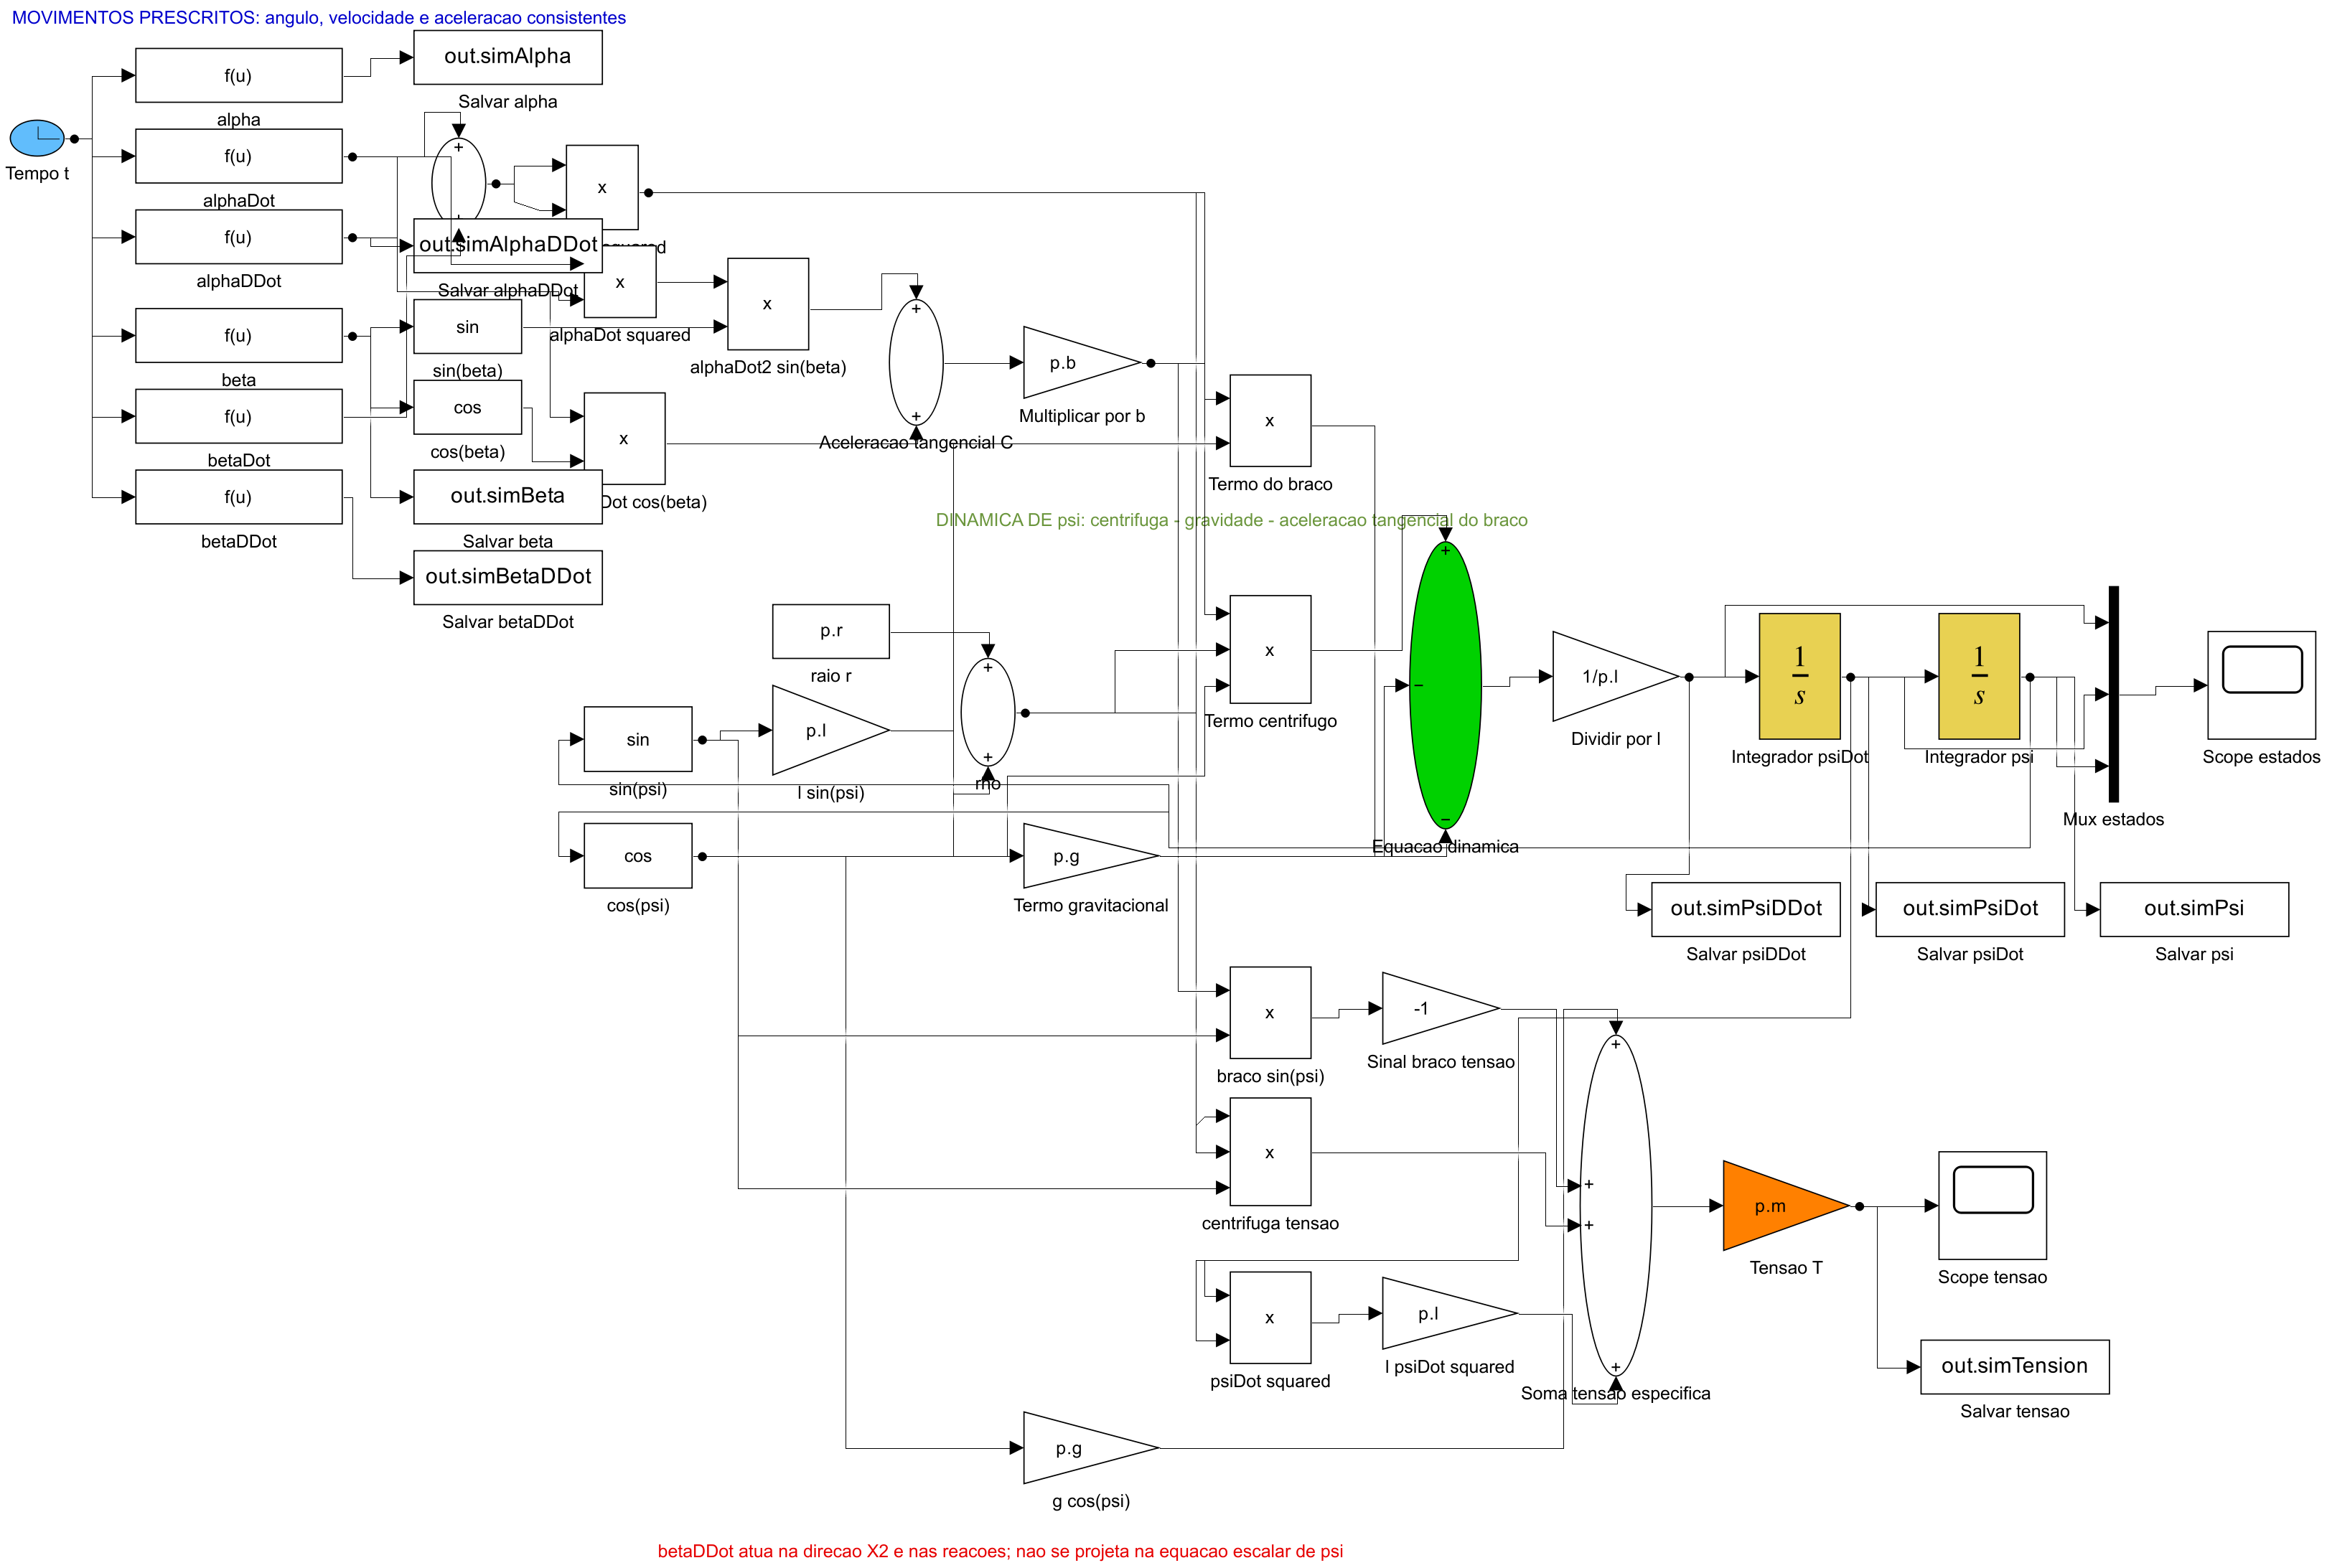
\includegraphics[width=\textwidth]{../docs/figures/simulink-diagram.png}
\caption{Implementação da equação diferencial com movimentos prescritos
acelerados.}
\label{fig:simulink}
\end{figure}

Com \texttt{ode45}, tolerâncias relativa e absoluta de $10^{-8}$ e $10^{-10}$
e passo máximo de \SI{0.01}{s}, a comparação com uma integração MATLAB
independente apresentou erros máximos de
$2{,}81\times10^{-10}\,\si{rad}$ em $\psi$ e
$1{,}30\times10^{-9}\,\si{rad.s^{-1}}$ em $\dot\psi$. A tração mínima foi
\SI{2.458}{N}. Com \texttt{ode4} e passo de \SI{0.002}{s}, os erros em relação
ao RK4 MATLAB foram $8{,}05\times10^{-16}\,\si{rad}$ e
$4{,}00\times10^{-15}\,\si{rad.s^{-1}}$, respectivamente.

O arquivo binário \texttt{.slx} é acompanhado por um gerador programático. Essa
duplicidade é deliberada: o modelo pode ser aberto diretamente para estudo e
também reconstruído a partir de uma fonte textual versionável.

\subsection{Modelo físico em Simscape Multibody}

O arquivo \texttt{rotating\_pendulum\_multibody.slx} representa a cadeia por
transformações rígidas, três juntas de revolução, gravidade, atuadores e
sensores. A massa $m$ é concentrada em $E$; os sólidos coloridos possuem massa
numérica desprezível para manter a correspondência com a hipótese de massa
pontual.

\begin{figure}[ht]
\centering
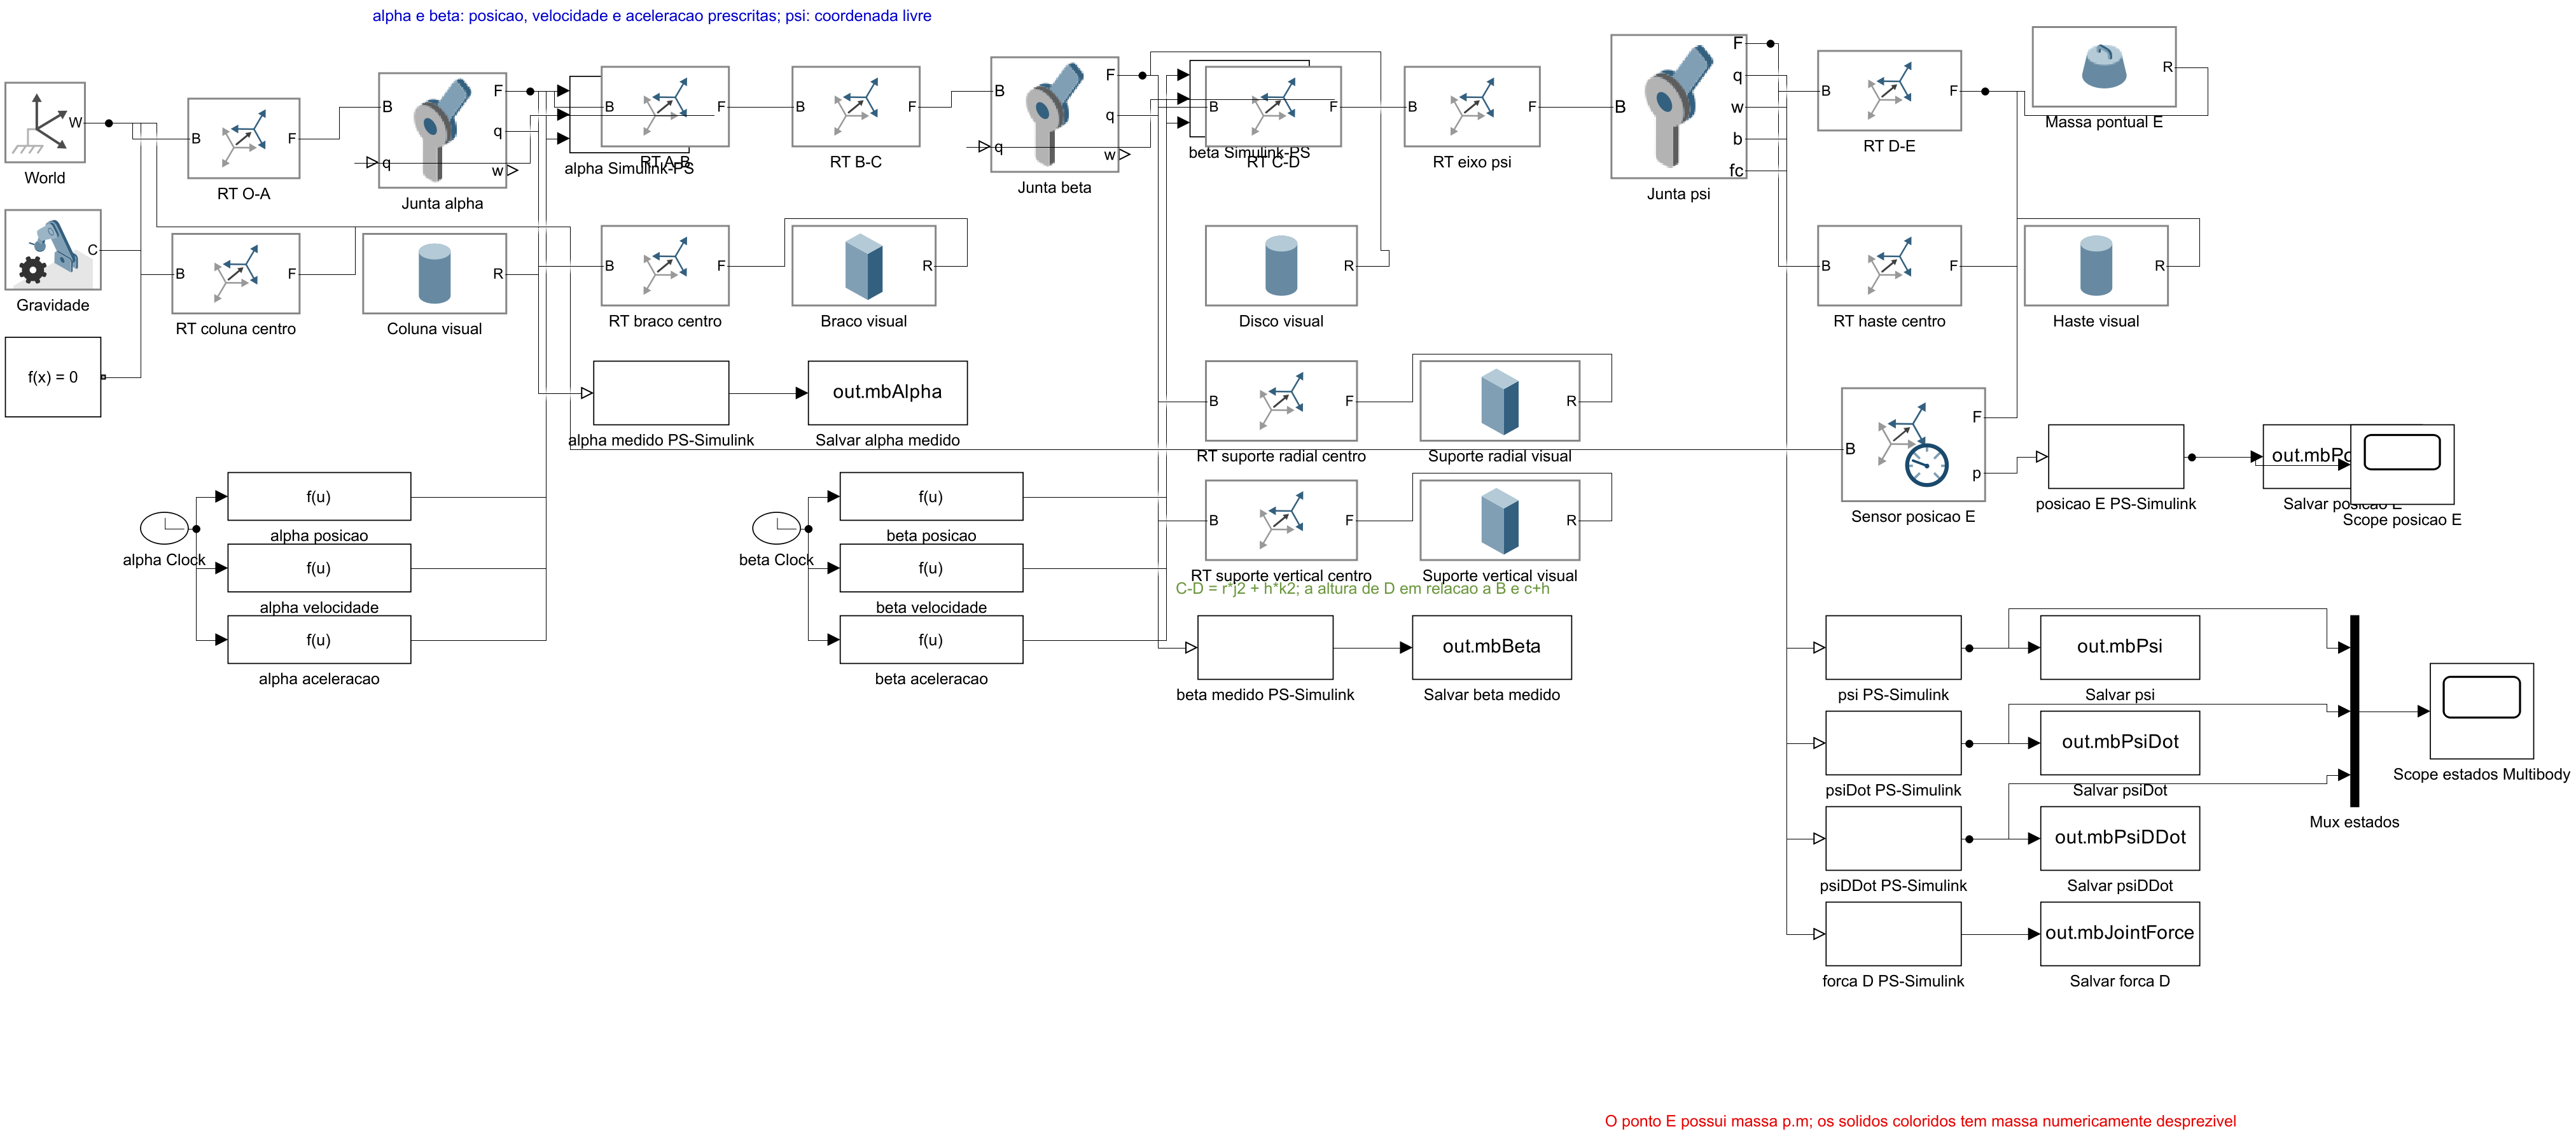
\includegraphics[width=\textwidth]{../docs/figures/multibody-diagram.png}
\caption{Modelo físico paramétrico em Simscape Multibody.}
\label{fig:multibody}
\end{figure}

Para cada junta acionada, o conversor físico recebe posição, velocidade e
aceleração calculadas pela mesma lei de movimento do modelo MATLAB. A junta de
$\psi$ permanece livre. Uma transformação rígida alinha o eixo padrão $Z$ da
junta com $X_2$, que é o eixo físico de oscilação.

A validação compara $\psi$, $\dot\psi$, $\ddot\psi$, a posição absoluta de $E$
e a força axial da haste. A força é obtida pela projeção da reação vetorial da
junta na direção instantânea de $DE$. Em \SI{20}{s}, os erros máximos foram
$7{,}76\times10^{-9}\,\si{rad}$ em $\psi$,
$3{,}71\times10^{-8}\,\si{rad.s^{-1}}$ em $\dot\psi$,
$2{,}72\times10^{-9}\,\si{m}$ na posição e
$1{,}15\times10^{-8}\,\si{N}$ na tração. A força axial mínima foi
\SI{2.458}{N}.

\begin{figure}[ht]
\centering
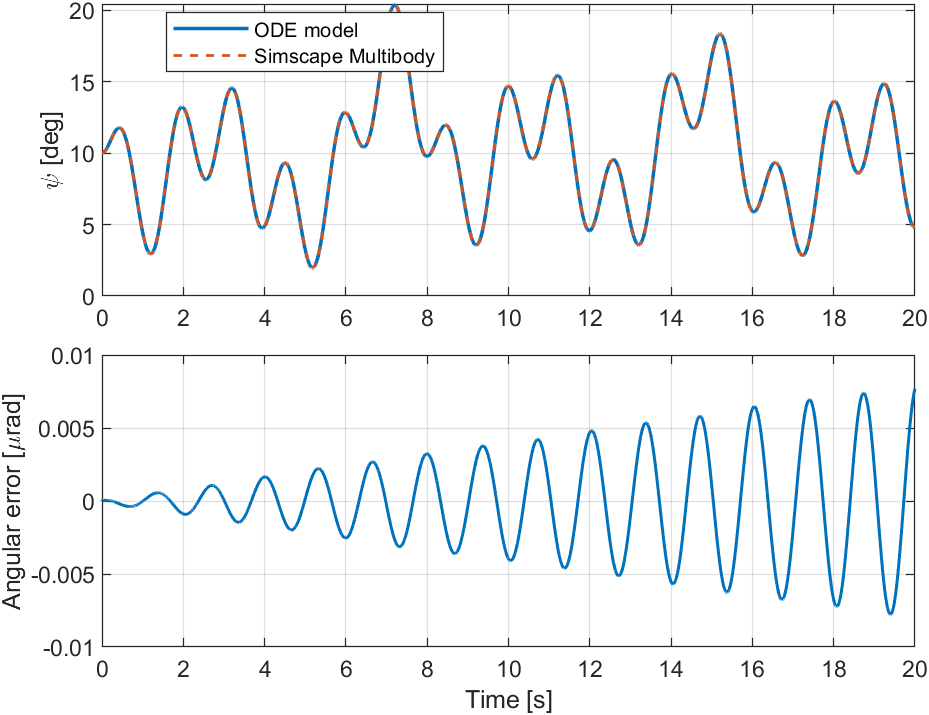
\includegraphics[width=0.88\textwidth]{../docs/figures/multibody-validation.png}
\caption{Comparação entre a equação de movimento e o modelo Multibody.}
\label{fig:multibody-validation}
\end{figure}

\subsection{Passagem para o modelo CAD}

Na integração futura, os sólidos paramétricos poderão ser substituídos por
blocos \texttt{File Solid} ou por uma montagem importada com \texttt{smimport}.
Os referenciais em $O$, $A$, $B$, $C$, $D$ e $E$ e as direções das juntas devem
ser mantidos. O mapeamento mínimo é apresentado na \cref{tab:cad-map}.

\begin{table}[ht]
\centering
\caption{Mapeamento entre a formulação e a montagem física.}
\label{tab:cad-map}
\begin{tabularx}{\textwidth}{@{}l l X@{}}
\toprule
Elemento & Modelo & Implementação física/virtual\\
\midrule
$OA$ & deslocamento $a\bvec k$ & coluna fixa\\
$AB$ & comprimento $b$, giro $\alpha$ em $Z$ & braço e junta acionada\\
$BC$ & deslocamento $c\bvec k$ & suporte vertical\\
$CD$ & $r\bvec j_2+h\bvec k_2$ & posição do pivô no disco\\
$DE$ & comprimento $l$, giro $\psi$ em $X_2$ & haste e junta pendular\\
$E$ & massa pontual $m$ & massa concentrada/centro de massa\\
\bottomrule
\end{tabularx}
\end{table}

Ao ativar massas e inércias reais, a resposta não deve mais coincidir
exatamente com a EDO de massa pontual. Nessa etapa, a formulação atual servirá
como caso de referência para avaliar o efeito da haste, do disco, das folgas e
dos atuadores reais.
\section{Conclusão}

O caso de velocidades constantes do exercício de referência foi preservado como
verificação, mas deixou de limitar o modelo. A formulação geral aceita
$\alpha(t)$ e $\beta(t)$ aceleradas e mostra com clareza a função de cada termo:
$\ddot\alpha$ altera diretamente a dinâmica de $\psi$, enquanto
$\ddot\beta$ contribui para a aceleração transversal e para as reações da junta.
A mesma lei de movimento alimenta MATLAB, Simulink e Simscape Multibody, evitando
a inconsistência comum de prescrever posição sem fornecer derivadas compatíveis.

Os testes cobrem a equação de movimento, a cinemática absoluta, o caso de
pêndulo simples e a comparação entre integradores. O modelo multicorpos mantém a
geometria $CD=r\bvec j_2+h\bvec k_2$ e pode receber peças CAD no lugar dos
sólidos paramétricos. Quando forem usadas massas e inércias reais, a equação de
massa pontual passará a ser uma referência simplificada, e não uma reprodução
completa do conjunto físico.
\appendix
\section{Parâmetros do caso demonstrativo}

\begin{table}[ht]
\centering
\begin{tabular}{@{}lll@{}}
\toprule
Parâmetro & Valor inicial & Observação\\
\midrule
$a$ & \SI{0.30}{m} & posição absoluta\\
$b$ & \SI{0.50}{m} & comprimento do braço\\
$c$ & \SI{0.10}{m} & posição absoluta\\
$r$ & \SI{0.20}{m} & distância radial no disco\\
$h$ & \SI{0.15}{m} & altura de $C$ a $D$\\
$l$ & \SI{0.35}{m} & comprimento do pêndulo\\
$m$ & \SI{0.25}{kg} & massa concentrada em $E$\\
$\bar\omega_\alpha$ & \SI{1.00}{rad.s^{-1}} & taxa média prescrita\\
$A_\alpha$ & \SI{0.20}{rad} & modulação de $\alpha$\\
$\nu_\alpha$ & \SI{0.80}{rad.s^{-1}} & frequência de modulação\\
$\bar\omega_\beta$ & \SI{1.60}{rad.s^{-1}} & taxa média relativa\\
$A_\beta$ & \SI{0.16}{rad} & modulação de $\beta$\\
$\nu_\beta$ & \SI{0.55}{rad.s^{-1}} & frequência de modulação\\
\bottomrule
\end{tabular}
\end{table}
Os valores servem apenas para tornar a simulação reproduzível. Dimensões,
massas, inércias e trajetórias de operação deverão ser substituídas pelos dados
do projeto CAD e dos atuadores antes de qualquer comparação experimental.

\end{document}
